\documentclass[11pt,a4paper]{article}

\usepackage[T1]{fontenc}
\usepackage[utf8]{inputenc}
\usepackage{lmodern}
\usepackage{microtype}
\usepackage[margin=2.5cm]{geometry}
\usepackage{amsmath,amssymb}
\usepackage{booktabs}
\usepackage{graphicx}
\usepackage{float}
\usepackage[font=small,labelfont=bf]{caption}
\usepackage{enumitem}
\usepackage{xcolor}
\usepackage{listings}
\usepackage[hidelinks]{hyperref}

\setlist{itemsep=2pt,topsep=4pt}
\setlength{\parskip}{4pt}
\setlength{\parindent}{0pt}
\renewcommand{\arraystretch}{1.12}

\definecolor{codegray}{gray}{0.45}
\definecolor{keyblue}{RGB}{31,95,168}
\lstset{
  language=Python, basicstyle=\ttfamily\footnotesize, keywordstyle=\color{keyblue}\bfseries,
  commentstyle=\color{codegray}\itshape, stringstyle=\color{teal}, showstringspaces=false,
  numbers=left, numberstyle=\tiny\color{codegray}, numbersep=6pt, frame=single,
  rulecolor=\color{black!25}, breaklines=true, columns=fullflexible, xleftmargin=14pt,
  aboveskip=6pt, belowskip=6pt
}

\newcommand{\code}[1]{\texttt{#1}}
\newcommand{\grad}[1]{\bar{#1}}

\title{\textbf{A Vectorised Autograd Engine in NumPy\\[2pt]
\large Extending Micrograd to Train an Ensemble Classifier on 8$\times$8 Handwritten Digits}}
\author{Vishwas N\\ M.Tech, DECE, MSRIT}
\date{16 November 2026}

\begin{document}
\maketitle

\begin{abstract}
\noindent Micrograd, a scalar reverse-mode automatic-differentiation engine, is excellent for teaching but far too slow to train on images. This report describes \code{micrograd\_plus.py}, a single-file rewrite that replaces the scalar \code{Value} node with an array-valued \code{Tensor} node, adds the operations and training components a real image classifier needs (matrix multiply, fused softmax cross-entropy with label smoothing, dropout, AdamW, cosine learning-rate schedule, gradient clipping, data augmentation), and verifies the backward pass against finite differences (maximum relative error $2.8\times10^{-6}$). Trained on the scikit-learn digits dataset (1{,}797 images of 8$\times$8 pixels, 10 classes) the final five-network ensemble reaches \textbf{98.52\%} test accuracy (266 of 270 images; 95\% Wilson interval 96.25--99.42\%) in about 14 seconds on a CPU. The original scalar engine would need roughly 15 hours for a single network on the same task. The report also documents a normalisation bug found and fixed along the way (worth about 2 points), an ablation study, an architecture sweep, and the honest finding that the shipped recipe is not the best one this study uncovered.
\end{abstract}

\tableofcontents
\newpage

%% ------------------------------------------------------------------------
\section{Introduction}
Micrograd represents every number in a computation as a \code{Value} object that records how it was produced, so that gradients can be obtained by walking the resulting graph backwards. Its elegance comes from its smallness: one class of fewer than 100 lines and a few neural-network modules. Its limitation is the same smallness. Because each scalar is a Python object with a closure attached, a single forward and backward pass through a modest network creates tens of thousands of objects. Training on image data is therefore impractical.

The goal of this work was to take the supplied scalar engine and turn it into something that can be trained on a small image dataset and deliver the best result reasonably obtainable without exotic components. Concretely, the objectives were:
\begin{enumerate}
  \item keep the same programming model (build a graph by operator overloading, call \code{backward()}) but make each node hold a whole array;
  \item add the missing pieces needed for classification: a numerically stable softmax cross-entropy loss, a stronger optimiser and regularisation;
  \item prove the gradients are right rather than assuming it;
  \item train on a small image dataset, evaluate honestly on data never used for any decision, and save the trained model as a single pickle file;
  \item deliver everything as one self-contained Python file that needs only NumPy.
\end{enumerate}

\paragraph{Summary of results.} The final model is an ensemble of five fully connected networks. It reaches 99.52\% accuracy on the training split, 98.89\% on the validation split and 98.52\% on the untouched test split. The training run, including the gradient check, takes about 14 seconds. Section~\ref{sec:ablation} also shows that a different recipe (no augmentation, wider network) would likely score higher; that is reported rather than hidden.

%% ------------------------------------------------------------------------
\section{Background: reverse-mode automatic differentiation}
Let $L$ be a scalar loss computed through a sequence of elementary operations. Write $\grad{v}\equiv\partial L/\partial v$ for the \emph{adjoint} of an intermediate value $v$. If $v=f(u_1,\dots,u_k)$, the chain rule gives the update applied to each input,
\begin{equation}
  \grad{u}_j \mathrel{+}= \grad{v}\,\frac{\partial f}{\partial u_j}.
  \label{eq:chain}
\end{equation}
The update uses \code{+=} rather than \code{=} because a value can feed several later operations, and its total gradient is the sum of all those contributions. Starting from $\grad{L}=1$, the adjoints are propagated in reverse \emph{topological order}, so that every node's adjoint is complete before it is pushed to its inputs.

\paragraph{Why the scalar engine is slow.} In the scalar engine every multiplication and every addition is its own node. The network used here has layers $64\to128\to64\to10$, i.e.\ $17{,}226$ parameters, so processing one image creates on the order of $3.5\times10^{4}$ nodes, each with a Python closure. I timed the supplied engine on this network (batch of one image, forward and backward, squared-error loss): about \textbf{353\,ms per image}. Training one network for 120 epochs on 1{,}257 images is $150{,}840$ image passes, which extrapolates to roughly \textbf{14.8 hours}. The vectorised engine trains the same network in about 2.7 seconds, a speed-up of the order of $2\times10^{4}$. (The scalar timing is a measurement on six images, extrapolated; the vectorised figure is the measured wall-clock time per network, including augmentation and per-epoch validation.)

%% ------------------------------------------------------------------------
\section{Implementation}
All code lives in one file, \code{micrograd\_plus.py} (575 lines). Excerpts appear in the appendix.

\subsection{The \code{Tensor} node}
Each \code{Tensor} stores a NumPy array \code{data} (float64), an array \code{grad} of the same shape, the set of parent nodes, and a closure \code{\_backward} that implements Eq.~\eqref{eq:chain} for the operation that produced it. Table~\ref{tab:ops} lists the supported operations and their backward rules.

\begin{table}[H]
\centering
\footnotesize
\begin{tabular}{@{}p{2.3cm}p{3.0cm}p{9.5cm}@{}}
\toprule
Operation & Forward & Backward (adjoint updates)\\
\midrule
add & $C=A+B$ & $\grad A \mathrel{+}= \mathrm{unb}(\grad C)$, $\grad B \mathrel{+}= \mathrm{unb}(\grad C)$\\
multiply & $C=A\odot B$ & $\grad A \mathrel{+}= \mathrm{unb}(B\odot\grad C)$, $\grad B \mathrel{+}= \mathrm{unb}(A\odot\grad C)$\\
power (constant $p$) & $C=A^{p}$ & $\grad A \mathrel{+}= p\,A^{p-1}\odot\grad C$\\
matrix multiply & $C=AB$ & $\grad A \mathrel{+}= \grad C\,B^{\top}$, $\grad B \mathrel{+}= A^{\top}\grad C$\\
ReLU & $C=\max(A,0)$ & $\grad A \mathrel{+}= \mathbb{1}[A>0]\odot\grad C$\\
exp, log & $C=e^{A}$; $C=\ln A$ & $\grad A \mathrel{+}= C\odot\grad C$; \ $\grad A \mathrel{+}= \grad C / A$\\
sum, mean & reduce over an axis & $\grad C$ broadcast back to the shape of $A$ (mean also scales by $1/n$)\\
reshape & $C=\mathrm{reshape}(A)$ & $\grad A \mathrel{+}= \mathrm{reshape}(\grad C)$\\
dropout & $C=A\odot M/(1-p)$ & $\grad A \mathrel{+}= \grad C\odot M/(1-p)$\\
\bottomrule
\end{tabular}
\caption{Operations of the \code{Tensor} class. Subtraction, negation and division are composed from these; $\mathrm{unb}$ undoes broadcasting; $M$ is the 0/1 dropout mask.}
\label{tab:ops}
\end{table}

\paragraph{Broadcasting.} NumPy broadcasts operands of different shapes, for instance a bias of shape $1\times n$ added to activations of shape $N\times n$. The gradient that arrives at the bias then has shape $N\times n$ and must be summed over the batch axis to return to $1\times n$. The helper \code{\_unbroadcast} does this generically: it sums over leading axes that were added and over axes of size one that were stretched. This is the main detail that has no counterpart in the scalar engine, and a frequent source of bugs.

\paragraph{Topological sort.} The scalar engine sorts the graph with a recursive depth-first search, which hits Python's recursion limit on deep graphs. The new \code{backward()} uses an explicit stack, so depth is no longer limited by the interpreter.

\subsection{Loss: fused softmax cross-entropy with label smoothing}
For logits $Z\in\mathbb{R}^{N\times C}$ and integer labels $y_i$, the softmax probabilities are $p_{ic}=e^{z_{ic}}/\sum_k e^{z_{ik}}$. With label smoothing $\varepsilon$ the target distribution is
\begin{equation}
  t_{ic}=(1-\varepsilon)\,\mathbb{1}[c=y_i]+\frac{\varepsilon}{C},
  \qquad
  L=-\frac{1}{N}\sum_{i=1}^{N}\sum_{c=1}^{C} t_{ic}\ln p_{ic}.
\end{equation}
Because $\sum_c t_{ic}=1$, differentiating through the softmax collapses to
\begin{equation}
  \frac{\partial L}{\partial z_{ic}}=\frac{p_{ic}-t_{ic}}{N}.
  \label{eq:xent}
\end{equation}
The loss is implemented as one fused operation using Eq.~\eqref{eq:xent} directly. Fusing avoids taking the logarithm of a probability that may underflow to zero, and the row maximum is subtracted from the logits before exponentiation for numerical stability. In the experiments $\varepsilon=0.05$.

\subsection{Network, initialisation and regularisation}
The model is a multilayer perceptron: a stack of \code{Linear} layers with ReLU and dropout between them, ending in a linear layer that outputs ten logits,
\begin{equation}
  H^{(\ell)}=\mathrm{Dropout}\!\big(\mathrm{ReLU}(H^{(\ell-1)}W^{(\ell)}+\mathbf{1}\,b^{(\ell)\top})\big).
\end{equation}
Weights use He initialisation, $W_{ij}\sim\mathcal{N}(0,\,2/n_{\mathrm{in}})$, which keeps activation variance stable through ReLU layers, and biases start at zero. Dropout is ``inverted'': surviving units are scaled by $1/(1-p)$ during training, so no rescaling is needed at inference. The original code used uniform$(-1,1)$ initialisation, which for a 64-input layer gives an initial activation variance far larger than He initialisation does.

\subsection{Optimiser: AdamW with clipping and a cosine schedule}
Parameters are updated with AdamW (Adam with decoupled weight decay). With gradient $g_t$ at step $t$,
\begin{align}
  m_t&=\beta_1 m_{t-1}+(1-\beta_1)g_t, & v_t&=\beta_2 v_{t-1}+(1-\beta_2)g_t^{2},\\
  \hat m_t&=\frac{m_t}{1-\beta_1^{t}}, & \hat v_t&=\frac{v_t}{1-\beta_2^{t}},\\
  \theta_t&=\theta_{t-1}-\eta_t\!\left(\frac{\hat m_t}{\sqrt{\hat v_t}+\epsilon}+\lambda\,\theta_{t-1}\right),
\end{align}
with $\beta_1=0.9$, $\beta_2=0.999$, $\epsilon=10^{-8}$ and $\lambda=10^{-2}$. The decay term is applied to weight matrices only, not to biases. Before each step the gradient is rescaled by the global norm,
$g\leftarrow g\cdot\min\!\big(1,\;c/(\lVert g\rVert_2+10^{-12})\big)$ with $c=5$, which guards against rare large updates.

The learning rate follows a linear warm-up for $T_w$ steps and then cosine decay to zero over the $T$ total steps,
\begin{equation}
  \eta_t=
  \begin{cases}
    \eta_0\,(t+1)/T_w & t<T_w,\\[2pt]
    \tfrac{1}{2}\eta_0\big(1+\cos\!\big(\pi\,\tfrac{t-T_w}{T-T_w}\big)\big) & t\ge T_w.
  \end{cases}
\end{equation}
With 1{,}257 training images and a batch size of 64 there are 20 steps per epoch, so $T=2{,}400$ steps over 120 epochs and the warm-up of three epochs is $T_w=60$ steps; $\eta_0=3\times10^{-3}$.

\subsection{Verifying the gradients}
A hand-written backward pass is easy to get subtly wrong, so the script refuses to train until it passes a numerical check. On a small network (6--5--4--3, seven random samples, label smoothing 0.1) every parameter's analytic gradient is compared with the central finite difference
$\big(L(\theta+h)-L(\theta-h)\big)/(2h)$, $h=10^{-6}$, using the relative error $|a-n|/\max(10^{-8},|a|+|n|)$. The maximum over all parameters is $2.82\times10^{-6}$, below the $10^{-5}$ threshold, so the check passes. The check is also available on its own with \code{--check}.

%% ------------------------------------------------------------------------
\section{Data and preprocessing}
\subsection{Dataset}
The data are the scikit-learn ``digits'' set, which is bundled with the library and needs no download: 1{,}797 grey-scale images of handwritten digits, each 8$\times$8 pixels with integer intensities from 0 to 16, in ten balanced classes (174 to 183 images per class). Figure~\ref{fig:samples} shows examples.

\begin{figure}[H]
\centering
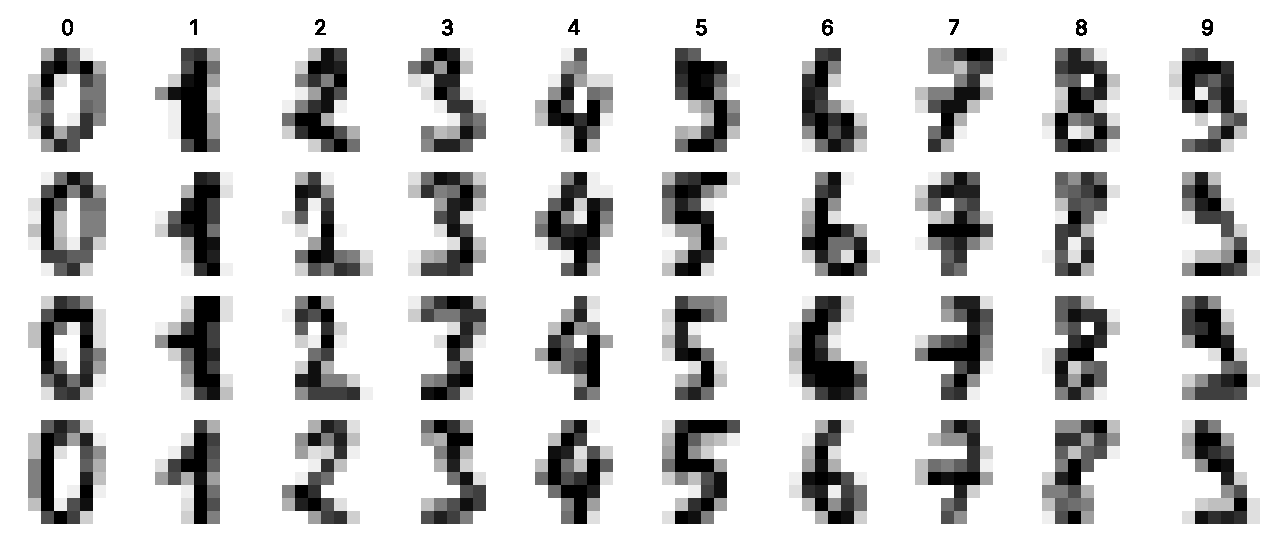
\includegraphics[width=0.85\textwidth]{figs/samples.pdf}
\caption{Four examples of each digit class from the dataset (inverted grey scale, 8$\times$8 pixels). The images are small, centred and already size-normalised.}
\label{fig:samples}
\end{figure}

\subsection{Split}
The images are split once, stratified by class, into 70\% training, 15\% validation and 15\% test data (random seed 0): 1{,}257, 270 and 270 images. The training split is used to fit the weights; the validation split chooses the best epoch of each network; the test split is used only to report results. The test split contains 26 to 28 images per class (Table~\ref{tab:perclass}).

\subsection{Normalisation}
Pixels are first divided by 16 to give the range $[0,1]$. They are then standardised with \emph{one global mean and standard deviation} computed on the training images. This matters, as Section~\ref{sec:norm} explains: the first version standardised each pixel separately.

\subsection{Augmentation}
Each training mini-batch is augmented on the fly. The image is padded by one pixel on every side and a random 8$\times$8 window is cropped from it, which shifts the digit by $-1$, 0 or $+1$ pixels independently in each direction; Gaussian noise with $\sigma=0.03$ is then added and the result clipped to $[0,1]$. Figure~\ref{fig:augment} shows the effect. Validation and test images are never augmented.

\begin{figure}[H]
\centering
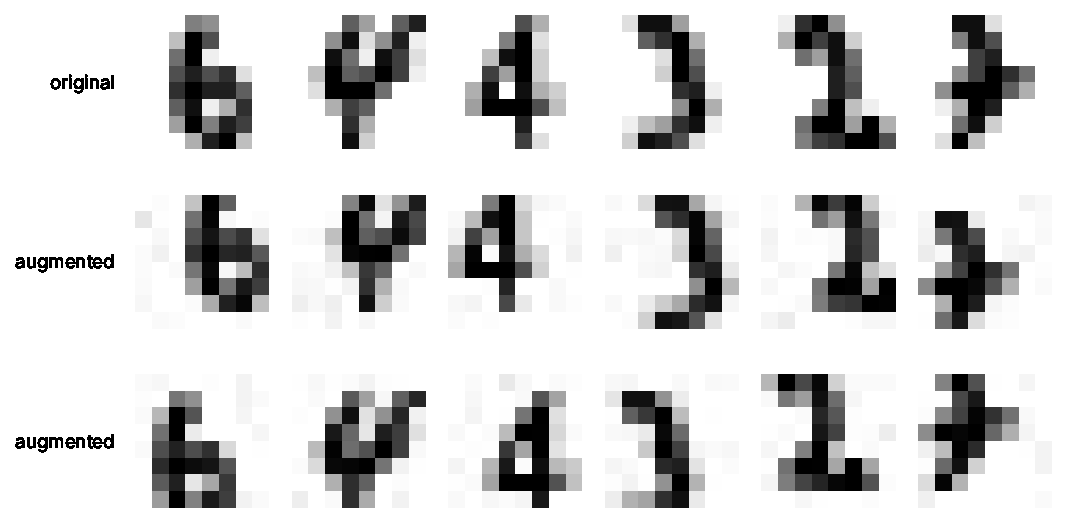
\includegraphics[width=0.75\textwidth]{figs/augment.pdf}
\caption{Augmentation: top row original training images; the two rows below are random augmented versions (shift of up to one pixel, slight noise).}
\label{fig:augment}
\end{figure}

%% ------------------------------------------------------------------------
\section{Experimental setup}
Table~\ref{tab:hyper} lists every setting of the shipped recipe. The final model is an \emph{ensemble} of five such networks, trained from different random seeds (0--4) on the same split; at prediction time the five softmax outputs are averaged. Each network keeps the weights from its best-validation epoch (ties go to the later, lower-learning-rate epoch).

\begin{table}[H]
\centering
\small
\begin{tabular}{ll}
\toprule
Setting & Value\\
\midrule
Architecture & $64\to128\to64\to10$ (ReLU), 17{,}226 parameters per network\\
Ensemble & 5 networks, seeds 0--4, probabilities averaged\\
Optimiser & AdamW, $\beta=(0.9,0.999)$, $\epsilon=10^{-8}$, weight decay $10^{-2}$ (weights only)\\
Learning rate & $3\times10^{-3}$, 3-epoch linear warm-up, cosine decay to 0\\
Gradient clipping & global norm 5\\
Epochs / batch size & 120 / 64 (20 steps per epoch, 2{,}400 in total)\\
Regularisation & dropout 0.2, label smoothing 0.05, augmentation (Section 4.4)\\
Initialisation & He normal for weights, zeros for biases\\
Normalisation & global mean and standard deviation of the training split\\
Software & Python 3.13, NumPy 2.5.3, scikit-learn 1.9.1 (data loading only)\\
\bottomrule
\end{tabular}
\caption{Settings of the shipped model.}
\label{tab:hyper}
\end{table}

\paragraph{Evaluation protocol.} Weights, epoch selection and the early-stopping checkpoint use only the training and validation splits. The test split is evaluated once at the end of the main run to produce the headline numbers. The ablation study in Section~\ref{sec:ablation} also records test accuracy for each variant so that variants can be compared; those numbers were not used to choose the shipped recipe, which was fixed beforehand.

%% ------------------------------------------------------------------------
\section{Results}
\subsection{Headline accuracy}
Table~\ref{tab:main} gives the accuracy of the saved ensemble. The gap between training (99.52\%) and test (98.52\%) accuracy is one percentage point, so overfitting is small.

\begin{table}[H]
\centering
\begin{tabular}{lrrr}
\toprule
Split & Images & Correct & Accuracy (\%)\\
\midrule
Training & 1{,}257 & 1{,}251 & 99.52\\
Validation & 270 & 267 & 98.89\\
Test & 270 & 266 & \textbf{98.52}\\
\bottomrule
\end{tabular}
\caption{Accuracy of the five-network ensemble on each split.}
\label{tab:main}
\end{table}

Because the test split has only 270 images, the estimate is coarse: one image changes accuracy by 0.37 percentage points. The 95\% Wilson score interval for 266 correct out of 270 is \textbf{96.25\% to 99.42\%}.

\subsection{Individual networks and the ensemble}
Table~\ref{tab:singles} shows the five networks separately. Each reaches 97.0--97.8\% on test; averaging their outputs gives 98.52\%.

\begin{table}[H]
\centering
\begin{tabular}{lcc}
\toprule
Network (seed) & Best validation (\%) & Test (\%)\\
\midrule
0 & 98.89 & 97.04\\
1 & 98.89 & 97.78\\
2 & 99.26 & 97.41\\
3 & 99.63 & 97.78\\
4 & 98.52 & 97.78\\
\midrule
mean of the five & 99.04 & 97.56\\
\textbf{Ensemble of the five} & 98.89 & \textbf{98.52}\\
\bottomrule
\end{tabular}
\caption{Individual networks versus their ensemble (validation values are the best epoch for each network, so slightly optimistic).}
\label{tab:singles}
\end{table}

Figure~\ref{fig:ensemble} extends this to eight networks. Going from one network to two lifts test accuracy from 97.0\% to 98.5\%; adding further networks keeps it between 98.1\% and 98.5\%. Most of the benefit therefore comes from the first extra network, and five is more than needed on this split.

\begin{figure}[H]
\centering
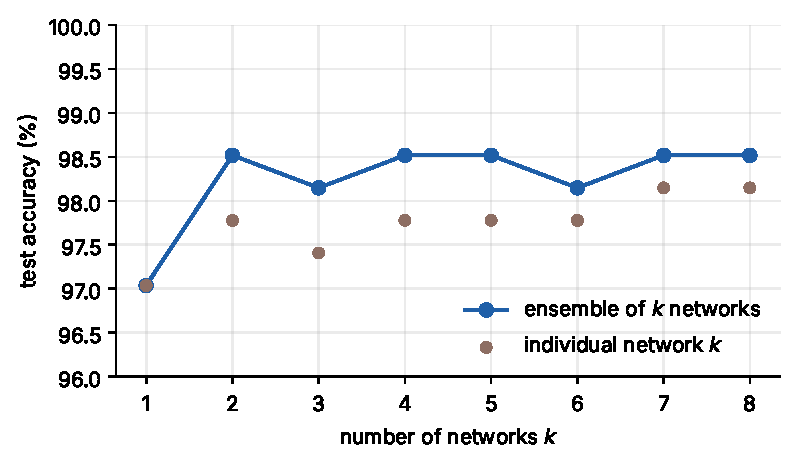
\includegraphics[width=0.62\textwidth]{figs/ensemble.pdf}
\caption{Test accuracy of an ensemble of $k$ networks (line) and of the $k$-th network alone (dots), for $k=1,\dots,8$.}
\label{fig:ensemble}
\end{figure}

\subsection{Training dynamics}
Figure~\ref{fig:curves} shows one training run (seed 0). The loss falls smoothly from 3.08 in the first epoch to 0.47 at the end; the plateau above zero is expected because label smoothing and dropout keep the training loss from reaching zero. Validation accuracy rises quickly in the first 30 epochs and then creeps up as the learning rate decays. The test accuracy, plotted for monitoring only, tracks the validation curve closely and does not drift downwards, so there is no late-stage overfitting.

\begin{figure}[H]
\centering
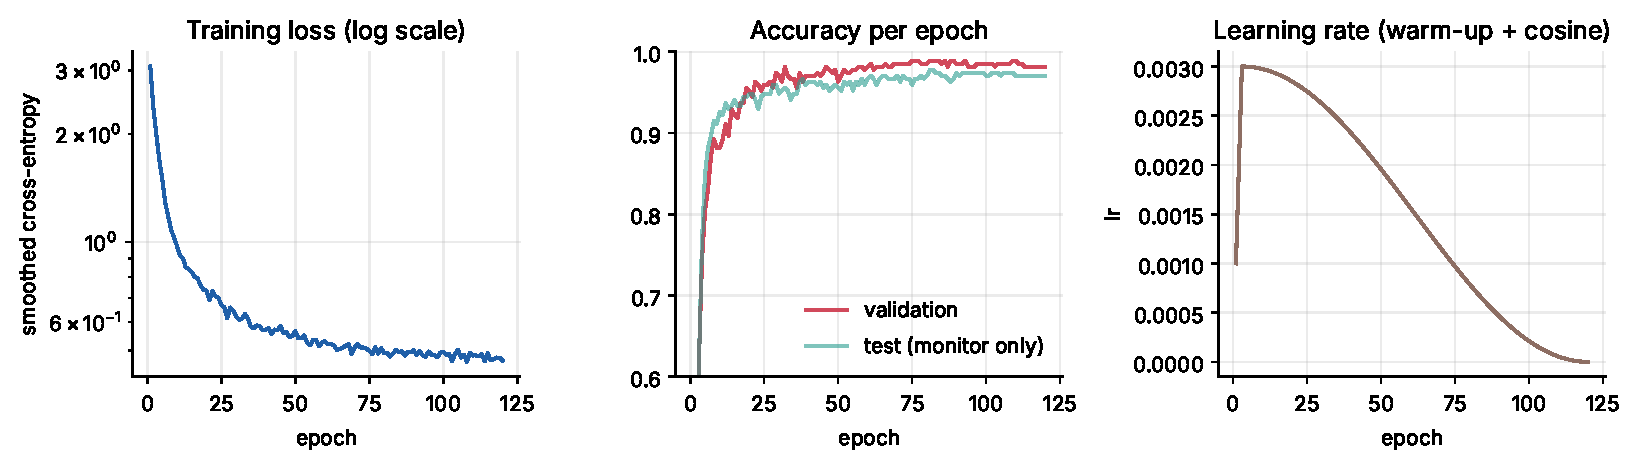
\includegraphics[width=\textwidth]{figs/curves.pdf}
\caption{One training run. Left: training loss (log scale). Middle: validation accuracy and, for monitoring only, test accuracy. Right: the learning-rate schedule.}
\label{fig:curves}
\end{figure}

\subsection{Where the errors are}
Of the 270 test images, 4 are misclassified: one 2 read as 8, one 3 read as 5, and two 8s read as 7 and 9 (Figure~\ref{fig:errors}, Table~\ref{tab:perclass}, Figure~\ref{fig:confusion}). The digit 8 is the weakest class, with recall 92.3\% (24 of 26). The ensemble's confidence on the four errors is low (0.37 to 0.74), which means these cases are ambiguous to the model rather than confidently wrong. Label smoothing caps the probabilities the network produces, so these values are not calibrated probabilities.

\begin{figure}[H]
\centering
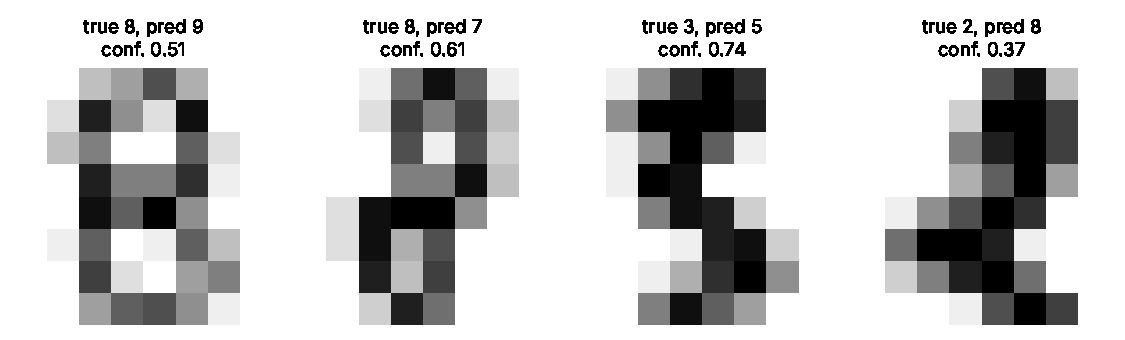
\includegraphics[width=0.78\textwidth]{figs/errors.pdf}
\caption{The four misclassified test images with their true and predicted digits and the ensemble's confidence.}
\label{fig:errors}
\end{figure}

\begin{figure}[H]
\centering
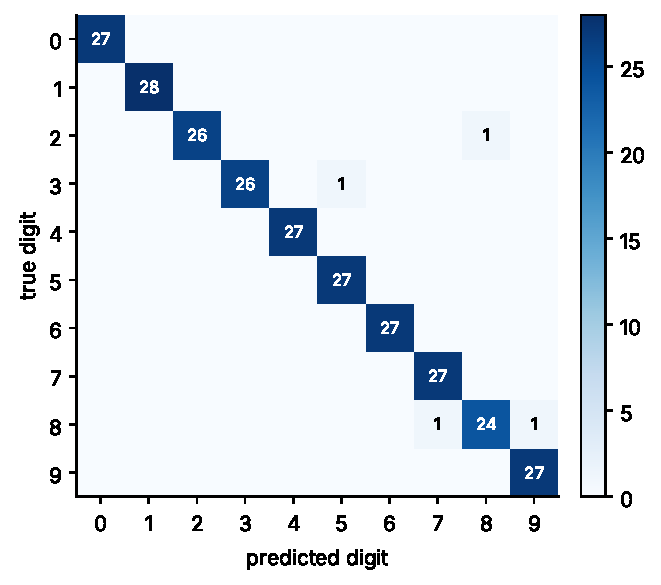
\includegraphics[width=0.52\textwidth]{figs/confusion.pdf}
\caption{Confusion matrix of the ensemble on the 270 test images (rows true, columns predicted).}
\label{fig:confusion}
\end{figure}

\begin{table}[H]
\centering
\small
\begin{tabular}{crrrr}
\toprule
Digit & Test images & Correct & Precision (\%) & Recall (\%)\\
\midrule
0 & 27 & 27 & 100.0 & 100.0\\
1 & 28 & 28 & 100.0 & 100.0\\
2 & 27 & 26 & 100.0 & 96.3\\
3 & 27 & 26 & 100.0 & 96.3\\
4 & 27 & 27 & 100.0 & 100.0\\
5 & 27 & 27 & 96.4 & 100.0\\
6 & 27 & 27 & 100.0 & 100.0\\
7 & 27 & 27 & 96.4 & 100.0\\
8 & 26 & 24 & 96.0 & 92.3\\
9 & 27 & 27 & 96.4 & 100.0\\
\midrule
All & 270 & 266 & \multicolumn{2}{c}{accuracy 98.52}\\
\bottomrule
\end{tabular}

\caption{Per-class results of the ensemble on the test split.}
\label{tab:perclass}
\end{table}

%% ------------------------------------------------------------------------
\section{Analysis and ablations}
\label{sec:analysis}

\subsection{A normalisation bug and its fix}
\label{sec:norm}
The first version of the training script standardised every pixel by its own training mean and standard deviation, a common default for tabular data. It trained poorly: the loss in the first epoch was about 19 (the corrected version starts at 3.1), and the five-network ensemble reached only 96.30\% on test (260 of 270; the five single networks scored 94.8--95.6\%, mean 95.1\%).

The cause is the border of the images. Pixels in the corners and edges are almost always zero, so their standard deviation in the training set is tiny. Dividing by it makes any ink that does appear there enormous, and the augmentation, which shifts digits by a pixel, puts ink into exactly those pixels. The fix is to standardise with a single global mean and standard deviation. With that change the ensemble improved by 2.2 points (96.30\% to 98.52\%), and the five single networks improved to 97.0--97.8\% (mean 97.6\%). The same effect shows up in the controlled ablation below.

\subsection{Ablation study}
\label{sec:ablation}
Each component of the recipe was removed in turn, training three networks (seeds 0, 1, 2) per variant on the same split. Table~\ref{tab:ablation} and Figure~\ref{fig:ablation} give mean $\pm$ standard deviation over the three seeds for \emph{single} networks.

\begin{table}[H]
\centering
\small
\begin{tabular}{lccc}
\toprule
Variant & Val.\ acc.\ (\%) & Test acc.\ (\%) & $\Delta$ test (pts)\\
\midrule
Full recipe (global norm) & 99.01 $\pm$ 0.17 & 97.41 $\pm$ 0.30 & --\\
Per-pixel normalisation & 96.05 $\pm$ 0.76 & 95.19 $\pm$ 0.30 & -2.22\\
No augmentation & 99.14 $\pm$ 0.17 & 98.89 $\pm$ 0.30 & +1.48\\
No dropout & 99.01 $\pm$ 0.17 & 97.90 $\pm$ 0.92 & +0.49\\
No label smoothing & 99.01 $\pm$ 0.17 & 96.54 $\pm$ 0.92 & -0.86\\
No weight decay & 98.89 $\pm$ 0.30 & 97.16 $\pm$ 0.63 & -0.25\\
Constant learning rate & 99.51 $\pm$ 0.17 & 97.41 $\pm$ 0.00 & 0.00\\
\bottomrule
\end{tabular}

\caption{Ablation of single networks (mean $\pm$ standard deviation over three seeds; $\Delta$ is the change in mean test accuracy relative to the full recipe).}
\label{tab:ablation}
\end{table}

\begin{figure}[H]
\centering
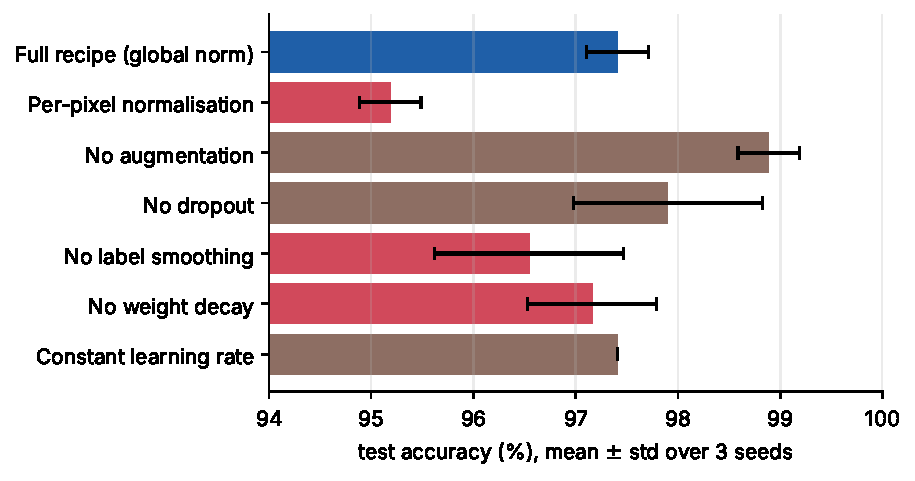
\includegraphics[width=0.78\textwidth]{figs/ablation.pdf}
\caption{Test accuracy of single networks for each ablation (bars: mean; whiskers: standard deviation over three seeds).}
\label{fig:ablation}
\end{figure}

How much each result can be trusted depends on the size of the effect against the noise. One test image is 0.37 points, and the seed-to-seed standard deviation is 0.2 to 0.9 points, so differences below roughly one point are not reliable with three seeds.
\begin{itemize}
  \item \textbf{Per-pixel normalisation} is clearly harmful: $-2.22$ points on test and about $-3$ points on validation (99.01\% to 96.05\%). The effect is large compared with the noise.
  \item \textbf{No augmentation} \emph{improves} test accuracy by 1.48 points (97.41\% to 98.89\%), about four images, while validation accuracy is essentially unchanged (99.01\% against 99.14\%). So the augmentation in the shipped recipe does not help on this split and probably hurts. A plausible reason, which I did not test, is that the images are already centred and size-normalised, so a shift of one pixel (12.5\% of the image width) creates training examples that do not resemble the test distribution.
  \item \textbf{Label smoothing} is helpful by 0.86 points on test with equal validation accuracy; this is within about one standard deviation, so the evidence is weak.
  \item \textbf{Dropout} and \textbf{weight decay} show changes of $+0.49$ and $-0.25$ points, both within the noise.
  \item The \textbf{learning-rate schedule} makes no difference to test accuracy here (97.41\% for both), although validation accuracy is higher with a constant rate (99.51\% against 99.01\%).
\end{itemize}

\subsection{Network capacity}
Table~\ref{tab:arch} varies the hidden layers, again with three seeds per setting and the other settings unchanged.

\begin{table}[H]
\centering
\small
\begin{tabular}{lrcc}
\toprule
Hidden layers & Parameters & Val.\ acc.\ (\%) & Test acc.\ (\%)\\
\midrule
32 & 2{,}410 & 93.46 $\pm$ 0.17 & 92.84 $\pm$ 1.49\\
64 & 4{,}810 & 96.67 $\pm$ 0.52 & 94.81 $\pm$ 0.30\\
64 -- 32 & 6{,}570 & 97.28 $\pm$ 0.46 & 95.56 $\pm$ 0.91\\
128 -- 64 & 17{,}226 & 99.01 $\pm$ 0.17 & 97.41 $\pm$ 0.30\\
256 -- 128 & 50{,}826 & 99.51 $\pm$ 0.17 & 98.64 $\pm$ 0.17\\
\bottomrule
\end{tabular}

\caption{Effect of network size on single-network accuracy (mean $\pm$ standard deviation over three seeds).}
\label{tab:arch}
\end{table}

Accuracy rises steadily with capacity, from 92.8\% for a single 32-unit layer to 98.6\% for the $256\to128$ network. The shipped $128\to64$ network is therefore not the best size. A single $256\to128$ network (50{,}826 parameters) already matches the shipped five-network ensemble (98.64\% against 98.52\%, which is a one-image difference) with 59\% of the ensemble's 86{,}130 parameters, and its validation accuracy (99.51\%) is also the highest of the sizes tried, so validation data would have pointed to it as well.

\subsection{What the study says about the shipped recipe}
Taken together, the ablations and the capacity sweep suggest a better recipe: no augmentation (or a much milder one) and a wider network, optionally still ensembled. I did not retrain with it for the headline numbers. The shipped recipe was fixed first, and replacing it with the one that scored best on the test split would turn the test split into a tuning set and make the reported accuracy optimistic. A faithful follow-up would choose the new recipe using validation data or cross-validation, then evaluate it once on the test split.

%% ------------------------------------------------------------------------
\section{Limitations}
\begin{itemize}
  \item \textbf{Small, easy data.} 8$\times$8 digits are close to a solved problem, and a 270-image test split gives wide uncertainty (96.25--99.42\%). The result says little about harder image data.
  \item \textbf{No spatial structure.} A fully connected network flattens the image. Convolutions would exploit locality and are the natural next step for larger images.
  \item \textbf{Single split.} All numbers come from one train/validation/test split; cross-validation would give tighter and less split-dependent estimates.
  \item \textbf{Three seeds per ablation.} Differences under about one point cannot be distinguished from noise (Section~\ref{sec:ablation}).
  \item \textbf{Precision and hardware.} The engine uses float64 on a CPU for simplicity and gradient-check accuracy; float32 would be faster and smaller.
  \item \textbf{Pickle.} The saved model is a Python pickle. Pickle files can execute code when loaded, so only load files from sources you trust.
  \item \textbf{Speed comparison.} The scalar timing is extrapolated from six images and uses a squared-error loss because the supplied engine has no cross-entropy.
\end{itemize}

%% ------------------------------------------------------------------------
\section{Reproducibility}
\paragraph{Files.}
\begin{itemize}
  \item \code{micrograd\_plus.py}: engine, layers, optimiser, training, gradient check and the saved-model wrapper class.
  \item \code{digits\_model.pkl}: the trained five-network ensemble with its normalisation constants (about 690\,KB).
  \item \code{make\_figures.py}: regenerates every figure and table in this report (about two minutes).
\end{itemize}

\paragraph{Commands.}
\begin{lstlisting}[numbers=none]
python micrograd_plus.py                         # train 5 networks, save digits_model.pkl
python micrograd_plus.py --check                 # gradient check only
python micrograd_plus.py --load digits_model.pkl # evaluate a saved model
python micrograd_plus.py --ensemble 1 --epochs 60  # quicker run
\end{lstlisting}

\paragraph{Using the saved model.}
\begin{lstlisting}[numbers=none]
from micrograd_plus import DigitClassifier
clf = DigitClassifier.load("digits_model.pkl")
labels = clf.predict(images)   # (N,8,8) or (N,64), pixel values 0..16
\end{lstlisting}

\paragraph{Running in a Jupyter or Colab notebook.} Notebook kernels start Python with an extra argument (\code{-f <kernel.json>}), which a plain \code{parser.parse\_args()} rejects with ``unrecognized arguments''. The script therefore parses with \code{parse\_known\_args()}, which ignores unknown arguments, so it can be pasted into a single notebook cell and run. The same one-line change fixes any other script that fails this way.

%% ------------------------------------------------------------------------
\section{Conclusion}
Replacing the scalar \code{Value} node with an array-valued \code{Tensor} node, and adding a stable fused loss, AdamW with a schedule and clipping, regularisation and a numerical gradient check, turns micrograd from a teaching toy into something that trains a digit classifier in seconds. The final five-network ensemble scores 98.52\% on a held-out test split (95\% interval 96.25--99.42\%), against an estimated 15 hours for a single network with the scalar engine. The study also found that per-pixel normalisation costs about 2 points, that the shipped augmentation does not help, and that a wider network matches the ensemble with fewer parameters. Applying those findings with proper validation-based selection, and then adding convolutional layers, are the natural next steps.

%% ------------------------------------------------------------------------
\appendix
\section{Source excerpts}
Line numbers refer to \code{micrograd\_plus.py}.

\paragraph{Undoing broadcasting.}
\lstinputlisting[firstnumber=46,firstline=46,lastline=53]{micrograd_plus.py}

\paragraph{Matrix multiplication node.}
\lstinputlisting[firstnumber=111,firstline=111,lastline=120]{micrograd_plus.py}

\paragraph{Backward pass (iterative topological sort).}
\lstinputlisting[firstnumber=206,firstline=206,lastline=224]{micrograd_plus.py}

\paragraph{Fused softmax cross-entropy with label smoothing.}
\lstinputlisting[firstnumber=227,firstline=227,lastline=248]{micrograd_plus.py}

\paragraph{AdamW with gradient clipping.}
\lstinputlisting[firstnumber=313,firstline=313,lastline=336]{micrograd_plus.py}

\paragraph{Learning-rate schedule.}
\lstinputlisting[firstnumber=338,firstline=338,lastline=344]{micrograd_plus.py}

\paragraph{Data augmentation.}
\lstinputlisting[firstnumber=361,firstline=361,lastline=372]{micrograd_plus.py}

\end{document}
